
\chapter{变率和微商}
从本章起,我们开始学习单变量的微积分学的基本概念和基础理论。

微积分学是研究变量的数学,变量之间的关系就是函数,因此,函数是微积分学研究的主要对象。

在函数的基本性质中,有两个最基本、最重要的概念-变率与求和,为了解决求函数的变率与求函数$f$在$[a,b]$上的和的问题就相应地产生微分与积分运算,而这两种运算之间,也存在着一种自然的互逆关系,在本章中,我们由函数的变率问题引出函数的微商(导数)概念,并给出初等函数的一套求导法则,在下一章中,我们揭示微分运算与积分运算的互逆关系,这就是微积分学的基本定理。

总起来说,微分反映了函数的局部性质,或在某个点附近的性质;积分则反映了函数的整体性质,或某个区间的性质;函数的局部性质与整体性质之间的有机联系,恰恰反映了微分运算与积分运算之间的互逆关系。

\section{微商(导数)的定义}
函数关系$y=f(x)$就是确定变量$y$如何随着变量$x$的变动而变动的关系,对于给定的函数$y=f(x)$, 变量$y$在变量$x$的不同点附近的变动情况是不尽相同的,这就是说,在变量$x$的
某个值$x_1$外,当$x_1$略加变动时,相应的$y$的变动可能相当剧烈(急增,或急减);而在变量$x$的另一个值$x_2$处,$y$的变动就可能较为迟缓,但是,用这样的语言来表达函数在某一点处的变率是不精确的,我们需要用“数量”来确切地表达这个意思,这就是函数在某点(或菜时刻)的变率的问题,简称变率。

\subsection{直线函数的变率}
一次函数$f (x) =kx+b$
是一种最简单的函数,它的函数图象是一条斜率等于$k$的直线,如图2.1所示。
\begin{figure}[htp]
    \centering
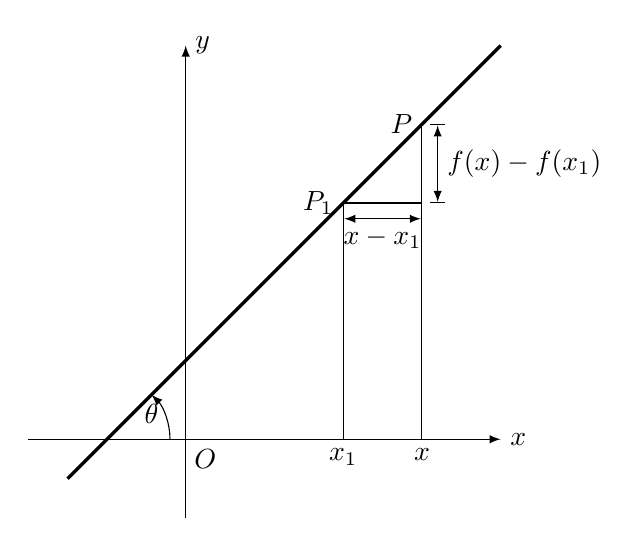
\begin{tikzpicture}[>=latex]
    \draw[->](-2,0)--(4,0)node[right]{$x$};
    \draw[->] (0,-1)--(0,5)node[right]{$y$};
    \draw[very thick] (-1.5,-.5)--(4,5);
\draw[->](-.2,0) arc (0:45:.8)node[below]{$\theta$};
\draw(2,3)node[left]{$P_1$}--(2,0)node[below]{$x_1$};
\draw(3,4)node[left]{$P$}--(3,0)node[below]{$x$};
\draw[|<->|](3.2,4)--node[right]{$f(x)-f(x_1)$}(3.2,3);
\draw[|<->|](2,2.8)--node[below]{$x-x_1$}(3,2.8);
\draw(2,3)--(3,3);\node at (.25,-.25){$O$};
\end{tikzpicture}
    \caption{}
\end{figure}

设$x_1$, $f(x_1)$和$x$, $f(x)$分别是直线上点$P_1$和$P$的坐标,为了反映函数变化快慢的问题,无论$x<x_1$还是$x>x_1$,自然地考虑在点$x_1$邻近,函数与自变量的相应的改变量的比:
\[\frac{f(x)-f(x_1)}{x-x_1}=\frac{(kx+b)-(kx_1+b)}{x-x_1}=k=\tan\theta\]
上面的表达式称为函数的\textbf{差商},它表示函数在区间$[x_1,x]$或$[x,x_1]$上对于自变量$x$的\textbf{平均变化率}。由于$k$是不随变量$x$变动而变动的常数,因此,一次函数在自变量的任何一个区间内的平均变化率都是常数。

如果让自变量的变化区间的长度无限地缩短,也就是让$x$无限地接近于$x_1$时,平均变化率所趋向的极限
\[\lim_{x\to x_1} \frac{f (x) -f (x_1)}{x-x_1} =k\]

\subsection{平滑曲线的切线与变率}
一般的函数$y=f(x)$的图象通常不是直线,由于函数
和它的图象的多样性,为了讨论的方便起见,我们先把讨论的范围限制在“平滑”的曲线上,常用的函数$y=f(x)$的图象往往是“平滑的”,平滑性的直观内涵是:用愈高倍的显微镜去观察曲线的微段,就愈象直线段,比较明确的几何说法是:一条曲线在$P$点的平滑性就是存在唯一的一条过$P$点的切线,它无限地逼近曲线在$P$点邻近的微段,于是,当$y=f(x)$的图象$C$在$P$点存在唯一的一条切线时,我们就说曲线$C$在$P$点平滑,而$P$点叫做曲线的平滑点,一条在每点都平滑的曲线叫做平滑的曲线,一个函数的图象平滑曲线时,我们就称这种函数为平滑函数。

同学可能会问这样一个问题:在曲线的点$P$存在唯一的一条切线的含义是什么?因为迄今我们对于一般的曲线的切
线还未下过定义呢!

我们从图2.2和2.3注意到不能把切线定义为与曲线只有一个交点的直线。这样的定义限制得既太紧同时又太松。因
为,照此定义,图2.2所示的直线就不是过曲线上$P$点的切线了,实际上,尽管图2.2的直线与曲线还有一个交点$Q$, 但它在曲
线$P$点邻近却与曲线密合,故仍应该是过曲线$P$点的切线;又图2.3表明过抛物线上任何一点$P$与$y$轴平行的直线虽然与抛物线只有一个交点,但它的其余部分却远离$P$点邻近的弧,故它不应该是抛物线的切线,定义切线的可行途径是从割线开始,并应用极限的概念。


如图2.4所示,取曲线$y=f(x)$上点$P$附近的另一点$Q$, 通过这两点画一条直线,这直线叫做过曲线上$P$点的割线,让$Q$点沿曲线向点$P$移动,这条割线将达到极限位置,此极限位置与$Q$点从哪一侧趋向于$P$是无关的,我们称这个割线的极限位置为过曲线上$P$点的切线。

割线的这种极限位置的存在性这一假设,与曲线在点$P$具有唯一的一条切线或确定的方向的假设是等价的。

现在我们要对曲线$y=f(x)$用解析式子把割线的这种极限位置存在的过程表示出来。
设$\alpha$是割线$PQ$同正$x$轴构成的夹角,$\alpha_1$是过点$P$点的切线同正$x$轴构成的夹角,于是
\[\lim_{Q\to P}\alpha=\alpha_1\]
设$x_1,y_1$和$x,y$分别是点$P$和$Q$的坐标,这时,我们立即得到
\[\tan\alpha=\frac{y-y_1}{x-x_1}=\frac{f(x)-f(x_1)}{x-x_1}\]
因此,上述求极限的过程(不考虑垂直切线$\alpha_1=\frac{\pi}{2}$的情况)可由下式来表示:
\[\lim_{x\to x_1}\frac{f(x)-f(x_1)}{x-x_1}=\lim_{\alpha\to \alpha_1}\tan\alpha=\tan\alpha_1\]
这就是说过曲线$y=f(x)$上$P(x_1,y_1)$点的切线的斜率等于$y=f(x)$的差商当$x\to x_1$时的极限.

\begin{example}
    求抛物线$y=ax^2+bx+c$在$x_0$处的切线的斜率。
\end{example}

\begin{solution}
    解依题意$(x_0,f(x_0)=ax_0^2+bx_0+c)$在抛物线上,并设$(x_0+h,f(x_0+h))$是抛物线上点$(x_0,f(x_0))$的附近的一点,我们有
\[\begin{split}
&\qquad \lim_{h\to 0}\frac{f(x_0+h)-f(x_0)}{(x_0+h)-x_0}\\
&=\lim_{h\to 0}\frac{[a(x_0+h)^2+b(x_0+h)+c]-[ax^2_0+bx_0+c]}{h}    \\
&=\lim_{h\to 0}\frac{(2ax_0+b)h+h^2}{h}\\
&=\lim_{h\to 0}[(2ax_0+b)+h]=2ax_0+b
\end{split}\]
所以抛物线$y=ax^2+bx+c$在$x_0$处的切线的斜率是$2ax_0+b$.
\end{solution}

\begin{example}
    一质点沿一直线在$t$秒内移动的距离是$s=s(t)=t^2+4t$。
    
    求:质点的初速度;在两秒末的速度;前两秒内的平均速度。
\end{example}

\begin{analyze}
    如果质点从起点开始所走的距离$s$是时间$t$的线性函数,则由2.1知道该质点在每一时刻的速度都是常数,它的大小由平均速度来确定,即等于一次函数的斜率,此时我们说该质点作匀速运动,但是,如果运动不再是匀速的,即质点的速度每时每刻都是变的,那么我们将时刻$t$的速度(也叫做瞬时速度)理解成什么呢?为了回答这个问题,我们考察差商
\[\frac{\Delta s}{\Delta t}=\frac{s(t)-s(t_0)}{t-t_0}\]
或者写成\[\frac{s(t_0+\Delta t)-s(t_0)}{\Delta t}\]
这个差商称为在$t_0$和$t_0+\Delta t$之间的这段时间间隔上的质点的平均速度,对照着$s=s(t)=t^2+4t$的图象来看,这个平均速度也就是过曲线上的$P(t_0,s(t_0))$
点及它邻近一点$Q(t_0+\Delta t,s(t_0+\Delta t))$的割线的斜率(图2.5)。当$\Delta t$ 很小时,可以认为,从时刻$t_0$到$t_0+\Delta t$这段时间内,速度来不及有很大变化,可以近似地看成匀速运动,因而这段时间内的平均速度就可以看成时刻$t_0$的瞬时速度的近似值。

\begin{figure}[htp]
    \centering
    \begin{tikzpicture}[>=latex, scale=.5]
\draw[->](-5.5,0)--(3,0)node[right]{$t$};
\draw[->](0,-5)--(0,7)node[right]{$s$};

\draw[domain=-5.25:0, samples=300, dashed]plot(\x, {\x*\x+4*\x});
\draw[domain=0:1.25, samples=100, thick]plot(\x, {\x*\x+4*\x});
\foreach \x in {-4,-3,-2,-1,1,2}
{
    \draw(\x,0)--(\x,.2);
}
\node at (-2,0)[below]{$-2$};
\node at (1,0)[below]{$1$};
\node at (0,0)[below left]{$O$};
    \end{tikzpicture}

    \caption{}
\end{figure}



显然,从时刻$t_0$到时刻$t_0+\Delta t$, 质点走过的路程为
\[\begin{split}
    \Delta s&=s(t_0+\Delta t)-s(t_0)\\
    &=(t_0+\Delta t)^2+4(t_0+\Delta t)+(t^2_0+4t_0)\\
    &=(2t_0+4)\Delta t+(\Delta t)^2
\end{split}\]
所以这段时间内的平均速度为
\[\begin{split}
    \frac{\Delta s}{\Delta t}&=\frac{s(t_0+\Delta t)-s(t_0)}{\Delta t}\\
    &=\frac{(2t_0+4)\Delta t+(\Delta t)^2}{\Delta t}\\
    &=(2t_0+4)+\Delta t
\end{split}\]
$\Delta t$越小,这个平均速度就越接近时刻$t_0$的瞬时速度$v_0$, 我们自然令$\Delta t\to 0$, 求差商的极限值,得到
\[\begin{split}
    \lim_{\Delta t\to 0}\frac{s(t_0+\Delta t)-s(t_0)}{\Delta t}&= \lim_{\Delta t\to 0}[(2t_0+4)+\Delta t]\\
    &=2t_0+4
\end{split}\]
这样平均速度$\frac{s(t_0+\Delta t)-s(t_0)}{\Delta t}$,当$\Delta t\to 0$时的极限值
就表达了质点在时刻$t_0$的瞬时速度,把它记作
\[s'(t_0)=   \lim_{\Delta t\to 0}\frac{s(t_0+\Delta t)-s(t_0)}{\Delta t}\]
\end{analyze}

\begin{solution}
\begin{enumerate}
\item 质点的初速度
\[s'(0)=2\x0+4=4(\ms)\]
\item 质点在两秒末的速度
\[s'(2)=2\x2+4=8(\ms)\]
\item \[\text{质点在前两秒内的平均速度}=\frac{\text{在前两秒内所走距离}}{\text{时间}}=\frac{2^2+4\x2}{2}
=6(\ms)\]
\end{enumerate}
\end{solution}

从这个问题可以看出质点在$t_0$时刻的瞬时速度$s'(t_0)$的几何意义就是曲线$s=s(t)$在$P(t_0,s(t_0))$点的切线的斜率,所以函数在某点的变率有确定值与函数的图象在该点有唯一的一条切线是两个密切相关的概念。

\subsection{微商(导数)的定义}
从上面所举的两个例子来看,问题来自不同的领域:
\begin{enumerate}
    \item 求过曲线上一点的切线,
    \item 求函数在某点的变率.
\end{enumerate}
但解决的方法却完全一样,就是计算函数的差商的极限,这种极限反映了自然界中很多不同现象在量方面的共性,因此有必要从这些具体问题中把它抽象出来加以研究,再反过来去解决这类具体问题。

\begin{blk}{定义}
    设$y=f(x)$是定义在闭区间$[a,b]$上的一个函数,$x_0\in (a,b)$, 如果极限
\[\lim_{\Delta x\to 0}\frac{f (x_0+\Delta x) -f (x_0)}{\Delta x}\]
存在,我们就说$f(x)$在点$x_0$处\textbf{可微},并称这极限为函数$f(x)$在$x_0$点的\textbf{微商}(或导数),记为$f'(x_0)$或
$\frac{\dd y}{\dd x}\Big|_{x=x_0}$.
\end{blk}

显然,$f'(x_0)$的值与点$x_0$有关,当点$x_0$在开区间$(a,b)$内变化时,$f'(x_0)$也将跟着变化,因此,如果函数$f(x)$在开区间$(a,b)$内每点都可微(即存在有限导数),那么$f'(x)$便是一个新的函数,称为$f(x)$的\textbf{导函数}。

求已知函数的导函数$f'(x)$的运算,称为微商 运算,计算过程如下:
\begin{enumerate}
\item 设$\Delta x$为自变量某个值$x$的改变量:
\item 计算$f(x)$在点$x$的相应改变量
\[\Delta y=f (x+\Delta x) -f (x) \]
\item 计算$f(x)$在点$x$的差商
\[\frac{\Delta y}{\Delta x}=\frac{f (x+\Delta x) -f (x)}{\Delta x}\]
\item 计算
\[\lim_{\Delta x\to 0}\frac{f (x+\Delta x) -f (x)}{\Delta x}=f'(x)=\frac{\dd y}{\dd x}\]
\end{enumerate}

应当注意,这里$\frac{\dd y}{\dd x}$是一个独立的记号,它表示函数$f(x)$
在点$x$的导数,不能把它当成一个分数来看待,必须把它看成一个整体。

从微商的定义可以看出:
\begin{enumerate}
\item 曲线在一点的切线的斜率,就是函数在这一点的变率(微商或导数)。    
\item 微商所涉及的是函数的“局部”性质,也就是说,函数$y=f(x)$在一点$x_0$处是否可微只与函数$y=f(x)$在$x=x_0$处及其近旁的性质有关,而与其它地方无关。    
\item 如果$f(x)$在点$x$可微,按照极限存在的条件,必须且只须
\[\lim_{\Delta x\to 0^+}\frac{f (x+\Delta x) -f (x)}{\Delta x},\qquad \lim_{\Delta x\to 0^-}\frac{f (x+\Delta x) -f (x)}{\Delta x}\]
同时存在而且相等。

上面两式分别称为$f(x)$在点$x$的\textbf{右导数}和\textbf{左导数},记为$f'_+(x)$和$f'_-(x)$.
\end{enumerate}

\begin{example}
今有一个正在膨胀的肥皂泡,
\begin{enumerate}
\item 求肥皂泡的体积对于半径的增大率,
\item 如果肥皂泡的半径每秒增大0.1cm,问当半径为2cm时,体积的增大率是多少?
\end{enumerate}
\end{example}

\begin{solution}
    肥皂泡的体积$V$与半径$r$的函数关系是。
\[ V(r) =\frac{4}{3}\pi r^3\]
体积$V(r)$对于半径$r$的增大率,依导函数定义,就是$V(r)$对于$r$的导函数,故
\[\begin{split}
    V'(r)&=\lim_{\Delta r\to 0}\frac{V(r+\Delta r)-V(r)}{\Delta r}\\
    &=\lim_{\Delta r\to 0}\frac{\frac{4\pi }{3}[(r+\Delta r)^3-r^3]}{\Delta r}\\
    &=\frac{4\pi }{3}\lim_{\Delta r\to 0}[3r^2+3r(\Delta r)+(\Delta r)^2]\\
    &=4\pi r^2
\end{split}\]

因此,肥皂泡的体积$V$对于半径$r$的增大率是$4\pi r^2$. 当$r=2$时,\[V'(2)=4\pi \cdot 2^2=16\pi \]
上式表示在$r=2$时,肥皂泡体积对于半径的增大率是$16\pi$, 它
的含义也可以这样理解,体积增大的快慢在$r=2$时,是$16\pi$倍于半径增大的快慢。

由于半径的增大率是每秒0.1cm,故体积在半径等于2时的增大率是
\[16\pi \x0.1=1.6\pi ({\rm cm^3/s})\]
\end{solution}

\begin{ex}
\begin{enumerate}
    \item 设$y=\frac{1}{x},\quad (x\ne 0)$,求
\begin{enumerate}
    \item 当$x$取改变量$\Delta x$后,函数改变量$\Delta y$的表达式;
    \item 当$x=3$, $\Delta x=-1$时,$\Delta y$的值;
    \item 当$x=3$时,$\frac{\Delta y}{\Delta x}$的表达式和$\frac{\dd y}{\dd x}\Big|_{x=3}$的值.
\end{enumerate}

    \item 设$\phi(x)=\frac{2}{x^2},\quad (x\ne0)$, 求
\begin{enumerate}
\item 当$x=1$, $\Delta x=-0.5$时,$\Delta \phi(x)$的值;
\item 对于任何$x\; (x\ne 0)$, 在$\Delta x$的间隔内,$\phi(x)$的平均变率$\frac{\Delta \phi}{\Delta x}$的表达式;
\item $\phi(x)$在任何点$x\; (x\ne 0)$处的瞬时变率$\phi'(x)$.
\end{enumerate}

    \item 平均变化率$\frac{\Delta y}{\Delta x}=\frac{f (x+\Delta x) -f (x)}{\Delta x}$依赖于哪两个变量?在平均变化率取极限求瞬时变化率的过程中,$x$是变量还是常量?$\Delta x$是变量还是常量?
    \item 点$P(2, 8)$在抛物线$y=x^2+2x$上,点$Q$为抛物线上任何一点。
\begin{enumerate}
    \item 求割线$PQ$的斜率的表达式;
  \item 当$Q$点横坐标为$2.1, 1.9, 2.002, 1.998, 2+h$时,求割线斜率的值;
\item 求在$P(2, 8)$点处,抛物线$y=x^2+2x$的切线方程和法线方程。
\end{enumerate}    

\item 求圆面积对于它的半径的变率,对于它的直径的变率.
\item 圆的半径的变率为2cm/s, 求圆面积在半径等于4cm
时的变率。
\end{enumerate}
\end{ex}

\subsection{函数的可微性与连续性的关系}

\begin{blk}
    {定理} 如果函数$f(x)$在点$x_0$可微,那么$f(x)$在点$x_0$处连续。
\end{blk}

\begin{proof}
设$f(x)$在点$x_0$处是可微的,也就是$f(x)$在$x_0$处有导数,则
\[f'(x_0)=\lim_{x\to x_0}\frac{f(x)-f(x_0)}{x-x_0}\]
所以
\[\begin{split}
    \lim_{x\to x_0}[f(x)-f(x_0)]&=\lim_{x\to x_0}\frac{f(x)-f(x_0)}{x-x_0}(x-x_0)\\
    &=\lim_{x\to x_0}\frac{f(x)-f(x_0)}{x-x_0}\cdot \lim_{x\to x_0}(x-x_0)\\
&=f'(x_0)\cdot 0=0
\end{split}\]
\end{proof}

上面的定理说明函数在其有导数的点一定连续,在其不
连续的点一定没有导数。但是它的逆命题不一定成立,即连续的函数不一定有导数。前面我们曾指出一个函数可微的充分必要条件是它的左导数和右导数都存在而且相等,下面给出在某些点不可微的函数的例子。

\begin{example}
    求函数$f(x)=|x^2-1|$的导函数的定义域。
\end{example}

    
\begin{solution}
函数$f(x)=|x^2-1|$是一个到处连续的函数,它的图象如图2.6所示.

去掉函数式中的绝对值的符号,$f(x)$便可以写成分段函数式:
\[f(x)=\begin{cases}
    x^2-1,& x\le -1\quad \text{或}\quad x\ge 1\\
    -(x^2-1), & -1\le x\le 1
\end{cases}\]
所以
\[f'(x)=\begin{cases}
    2x ,&  x< -1\quad \text{或}\quad x> 1\\
    -2x,& -1<x<1
\end{cases}\]
但是当$x=-1$和1时,函数$f(x)$的左导数和右导数不相等,即此时导数不存在。因为当$x=-1$时,函数$f(x)$在$-1$点左邻域的表达式是
\[f (x) =x^2-1\]
而在$-1$点右邻域的表达式是
\[f (x) =- (x^2-1)\]
所以$f(x)$在$x=-1$点的左导数是
\[\begin{split}
    f'_-(-1)&=\lim_{\Delta x\to 0^-}\frac{f(-1+\Delta x)-f(-1)}{\Delta x}\\
    &=\lim_{\Delta x\to 0^-}\frac{[(-1+\Delta x)^2-1]-0}{\Delta x}\\
    &=\lim_{\Delta x\to 0^-}(-2+\Delta x)=-2
\end{split}\]
$f(x)$在$x=-1$点的右导数是
\[\begin{split}
    f'_+(-1)&=\lim_{\Delta x\to 0^+}\frac{f(-1+\Delta x)-f(-1)}{\Delta x}\\
    &=\lim_{\Delta x\to 0^+}\frac{-[(-1+\Delta x)^2-1]-0}{\Delta x}\\
    &=\lim_{\Delta x\to 0^+}(2-\Delta x)=2 
\end{split}\]
由于$f'_-(-1)\ne f'_+(-1)$, 所以我们说$f(x)$在$x=-1$处的导数不存在,同样可得
\[-2=f'_- (1)\ne f'_+(1)=2\]
故$f(x)$在$x=1$处也不可微.

因此,$f(x)=|x^2-1|$的导函数的定义域是$x\ne\pm 1$的点的集合,它的函数值如下:
\[f'(x)=\begin{cases}
    2x,& |x|>1\\
    -2x,& |x|<1
\end{cases}\]
\end{solution}

对照图2.6来看,尽管函数$f(x)=|x^2-1|$处处连续,但是在$x=-1$和1这两点,曲线的特征是当动点由左侧趋于定
点1(或$-1$)时,割线的极限位置存在;当动点由右侧趋于定点1(或$-1$)时,割线的极限位置也存在,这两个极限位置分别叫1(或$-1$)点的\textbf{左、右切线},并且它们之间的夹角不为\textbf{平角},点$-1$和1分别是曲线的一种\textbf{角点}.
    
图2.7的情形是曲线$y=f(x)$在$P(x_0,y_0)$点连续并且在此点有平行于$y$轴的切线.现在我们来讨论图2.7中所示各函数在点$x_0$处的导数:

图(a)表示的函数在点$x_0$的邻近递增,因此过曲线上$P(x_0,y_0)$和$Q(x_0+\Delta x,y_0+\Delta y)$两点的割线,无论$Q$点在$P$点的哪一侧,$\Delta x$与$\Delta y$都有相同正、负号,于是
\[\frac{\Delta y}{\Delta x}=\frac{f(x_0+\Delta x)-f(x_0)}{\Delta x}>0\]
而且当$\Delta x\to 0$时,割线的倾斜角$\varphi$($0^{\circ}\le \varphi\le 180^{\circ}$)便以$\pi/2$为极限,从而
\[\lim_{\Delta x\to 0}\frac{f(x_0+\Delta x)-f(x_0)}{\Delta x}=\lim_{\varphi\to \tfrac{\pi^-}{2}}\tan\varphi=+\infty\]
可见$f(x)$在点$x_0$不可微(不存在有限导数),但是我们常常把这种情况:当$\Delta x\to 0$时,$\frac{\Delta y}{\Delta x}\to\infty$简略地叙述为函
数$f(x)$在$x_0$的导数为正无穷大,记作$f'(x_0)=+\infty$。

图(b)表示的函数$f$在点$x_0$的邻近递减,因此过曲线上$P(x_0,y_0)$和$Q(x_0+\Delta x,y_0+\Delta y)$两点的割线,无论$Q$点在$P$点的哪一侧,$\Delta x$与$\Delta y$都有相反的正、负号,于是
\[\frac{\Delta y}{\Delta x}=\frac{f(x_0+\Delta x)-f(x_0)}{\Delta x}<0\]
而且当$\Delta x\to 0$时,$\varphi\to \frac{\pi^+}{2}$,从而
\[\lim_{\Delta x\to 0}\frac{f(x_0+\Delta x)-f(x_0)}{\Delta x}=\lim_{\varphi\to \tfrac{\pi^+}{2}}\tan\varphi=-\infty\]
因此$f(x)$在点$x_0$处不可微,但是我们常常把这种情况叙述为函数$f(x)$在$x_0$处的导数为负无穷大,记作$f'(x_0)=-\infty$。

图2.7(c)表示的函数在点$x_0$处连续,让$x$由$x_0$变动到
$x_0+\Delta x$,于是由$\Delta x$所引起的相应的函数的改变量$\Delta y$的情形是:
\begin{itemize}
    \item 当$\Delta x<0$时,有$\Delta y<0$,从而$\frac{\Delta y}{\Delta x}>0$;
    \item 当$\Delta x>0$时,有$\Delta y<  0$,从而$\frac{\Delta y}{\Delta x}<0$。
\end{itemize}
于是:
\begin{itemize}
    \item 当$\Delta x\to 0^-$时,$\varphi\to \frac{\pi^-}{2}$,从而$\frac{\Delta y}{\Delta x}=\tan\varphi\to +\infty$;
    \item 当$\Delta x\to 0^+$时,$\varphi\to \frac{\pi^+}{2}$,从而$\frac{\Delta y}{\Delta x}=\tan\varphi\to -\infty$。
\end{itemize}
因此$f(x)$在点$x_0$不可微,但是我们常把这种情况叙述为$f(x)$在点$x_0$的左导数$f'_-(x_0)=+\infty$, 而它的右导数为$f'_+(x_0)=-\infty$, 曲线在$x_0$处由上升转为下降有一个尖点,它的切线垂直于$x$轴。

图(d)表示的函数在点$x_0$处连续,但是
\begin{itemize}
    \item 当$\Delta x\to 0^-$时,$\frac{\Delta y}{\Delta x}=\tan\varphi\to -\infty$;
    \item 当$\Delta x\to 0^+$时,$\frac{\Delta y}{\Delta x}=\tan\varphi\to +\infty$。
\end{itemize}
因此,$f(x)$在点$x_0$不可微,我们常常把这种情况叙述为$f'_-(x_0)=-\infty$和$f'_+(x_0)=+\infty$, 点$x_0$是曲线的一个尖点,它的切线垂直于$x$轴。

\begin{example}
设$f(x)=\begin{cases}
    0,& x=0\\
    x\sin\frac{1}{x},& x\ne 0
\end{cases}$

讨论它在0点的导数。
\end{example}

\begin{solution}
在第一章,我们已经说明了
\[\lim_{x\to 0}x\sin\frac{1}{x}=0=f(0)\]
因此,$f(x)$在点$x=0$连续,很明显$f(x)$在其它各点处也都连续,所以说$f(x)$是一个到处连续的函数,我们将说明它在原点不存在导数。

因为
\[\frac{f(0+\Delta x)-f(0)}{\Delta x}=\frac{\Delta x\sin\frac{1}{\Delta x}}{\Delta x}=\sin\frac{1}{\Delta x}\]
而当$\Delta x\to 0$时,$\sin\frac{1}{\Delta x}$
没有极限,故$f'(0)$不存在,就
其几何意义来说,当动点沿着曲线$y=x\sin\frac{1}{x}$趋于原点$O$
时,割线$OQ$不断地在$-\frac{\pi}{4}\le \theta\le \frac{\pi}{4}$这个幅度之内摆动,而不趋于任何极限位置,即切线不存在(图2.8)。
\end{solution}

通过以上的例子,我们知道函数的连续点未必是它的可以微分点。几种常见的不可微分点如例2.4的角点,平行于$y$轴的切线的切点,特别是曲线上的尖点和在例2.5的曲线上的不存在割线的极限位置的点。

假如区间$[a,b]$上的函数$f(x)$, 在开区间$(a,b)$中存在着导数$f'(x)$, 并且$f'_+(a)$和$f'_-(b)$都存在,则称$f(x)$在闭区间上可以微分(可导)。

\begin{ex}
\begin{enumerate}
    \item 说明下面函数在点$x=0$不可微:
\begin{multicols}{2}
\begin{enumerate}
    \item $f(x)=|x|$
    \item $f(x)=\begin{cases}
        x^2,& x\le 0\\
        x,& x\ge 0
    \end{cases}$
    \item $f(x)=\sqrt[3]{x}$
    \item $f(x)=\sqrt{|x|}$
\end{enumerate}
\end{multicols}
\item 说明函数$f(x)=\begin{cases}
    x^2,& x\ge 0\\
    -x^2,& x<0
\end{cases}$
    处处可微。
\item \begin{enumerate}
\item 假设$g(x)=f(x+c)$. 从定义出发证明$g'(x)=f'(x+c)$, 并绘图说明。    
\item 设$f$可微并有周期$\varphi$, 证明$f'$也是有周期的.
\end{enumerate}

\end{enumerate}
\end{ex}

\section{微商运算的基本法则}
\subsection{几个基本函数的微商(导数)}
\subsubsection{常数函数的导数恒等于0}

\begin{proof}
设$f(x)=c$ ($c$是常数),则根据常数函数的性质,由自变数$x$的改变量$\Delta x$引起的相应的函数的改变量为:
\[\Delta y=f (x+\Delta x) -f (x)=c-c=0\]
显然差商$\frac{\Delta y}{\Delta x}=\frac{0}{\Delta x}=0$, 故
\[f' (x) =\lim_{\Delta x\to 0}\frac{\Delta y}{\Delta x}=
\lim_{\Delta x\to 0} 0=0\]
这个事实是明显的,因为当自变数$x$有增、减时,函数值并无增、减,因此,它的变化率为零。
\end{proof}

\subsubsection{一次函数(直线函数)的导数是常数}

若$f(x)=kx+b$, 则$f'(x)=k$. 

\subsubsection{若$f(x)=x^n$ ($n$是正整数),则$f'(x)=nx^{n-1}$}

\begin{proof}
  由自变量的改变量$\Delta x$引起的函数改变量为
\[\Delta y=f (x+\Delta x) -f (x) = (x+\Delta x)^n-x^n\] 
按牛顿二项式定理展开,得  
\[\begin{split}
\Delta y&= x^n+nx^{n-1}\Delta x+\frac{n(n-1)}{1\cdot 2}x^{n-2}(\Delta x)^2+\cdots+nx(\Delta x)^{n-1}+(\Delta x)^n-x^n\\
&=nx^{n-1}\Delta x+\frac{n(n-1)}{1\cdot 2}x^{n-2}(\Delta x)^2+\cdots+nx(\Delta x)^{n-1}+(\Delta x)^n
\end{split}\]
其中差商
\[\frac{\Delta y}{\Delta x}=nx^{n-1}+\frac{n(n-1)}{1\cdot 2}x^{n-2}\Delta x+\cdots+nx(\Delta x)^{n-2}+(\Delta x)^{n-1}\]
式中除第一项外,其余各项随$\Delta x\to 0$而趋于0,因此:
\[f'(x)=\lim_{\Delta x\to 0}\frac{\Delta y}{\Delta x}=nx^{n-1}\]
\end{proof}

\subsubsection{若$f(x)=x^{\mu}$ (其中$\mu$是任意实数,函数的定义域依赖于$\mu$), 则$f'(x)=\mu x^{\mu-1}$}

\begin{proof}
    \[\frac{\Delta y}{\Delta x}=\frac{(x+\Delta x)^{\mu}-x^{\mu}}{\Delta x}=x^{\mu-1}\cdot \frac{\left(1+\frac{\Delta x}{x}\right)^{\mu-1}}{\frac{\Delta x}{x}}\]
利用第一章中已经算出的极限
\[\lim_{x\to 0}\frac{(1+x)^{\mu}-1}{x}=\mu\]
就得到
\[f'(x)=\lim_{\Delta x\to 0}\frac{\Delta y}{\Delta x}=\mu x^{\mu-1}\]
\end{proof}

特殊情形:
\begin{enumerate}
    \item 若$f(x)=\frac{1}{x}=x^{-1},\; (x\ne 0)$,则$f'(x)=(-1)x^{-2}=-\frac{1}{x^2}$
    \item 若$f(x)=\sqrt{x}=x^{\tfrac{1}{2}},\; (x\ge 0)$,则$f'(x)=\frac{1}{2}x^{-\tfrac{1}{2}}=\frac{1}{2\sqrt{x}}$
\end{enumerate}

\subsubsection{若$f(x)=\log_a x\; (0<a\ne 1,\; 0<x<+\infty)$,则$f'(x)=\frac{\log_a e}{x}$}

\begin{proof}
\[\begin{split}
    \frac{\Delta y}{\Delta x}&=\frac{\log_a(x+\Delta x)-\log_a x}{\Delta x}\\
    &=\frac{1}{x}\cdot \frac{\log_a\left(1+\frac{\Delta x}{x}\right)}{\frac{\Delta x}{x}}\\
    &=\frac{1}{x}\cdot \log_a\left(1+\frac{\Delta x}{x}\right)^{\tfrac{1}{\Delta x/x}}
\end{split}\]  

利用极限$\Lim_{t\to 0}(1+t)^{1/t}=e$,以及对数函数是连续函数,得到
\[\begin{split}
    f'(x)&=\lim_{\Delta x\to 0}\frac{\Delta y}{\Delta x}=\frac{1}{x}\lim_{\tfrac{\Delta x}{x}\to 0}\log_a\left(1+\frac{\Delta x}{x}\right)^{\tfrac{1}{\Delta x/x}}\\
    &=\frac{1}{x}\log_a\left[\lim_{\tfrac{\Delta x}{x}\to 0}\left(1+\frac{\Delta x}{x}\right)^{\tfrac{1}{\Delta x/x}}\right]\\
    &=\frac{1}{x}\log_a e=\frac{\log_a e}{x}
\end{split}\]

特别:当$f(x)=\ln x$时,$f'(x)=\frac{1}{x}$。
\end{proof}

上面的结果表明对数函数($a>1$时)的增大速度是与自
变数的值成反比的,当自变数无限增大时,增大速度就保持正值而趋向于0. 由于自然对数的导数比较简单,所以在理论研究中常常采用自然对数。

\subsubsection{若$f(x)=a^x\; (0<a\ne 1,\; -\infty<x<+\infty)$,则$f'(x)=a^x\cdot \ln a$}

\begin{proof}
    \[\frac{\Delta y}{\Delta x}=\frac{a^{x+\Delta x}-a^x}{\Delta x}=a^x\cdot \frac{a^{\Delta x}-1}{\Delta x}\]
利用$\Lim_{\Delta x\to 0}a^{\Delta x}=1$,则可设$a^{\Delta x}=1+\alpha$,且当$\Delta x\to 0$时,有$\alpha\to 0$. 在此等式的两边取对数,得:
\[\Delta x=\log_a(1+\alpha)\]
于是
\[\frac{\Delta y}{\Delta x}=a^x\cdot \frac{\alpha}{\log_a(1+\alpha)}=a^x\cdot \frac{1}{\log_a(1+\alpha)^{1/\alpha}}\]
因此
\[\begin{split}
    f'(x)&=\lim_{\Delta x\to 0}\frac{\Delta y}{\Delta x}=a^x\cdot \frac{1}{\Lim_{\alpha\to 0}\log_a(1+\alpha)^{1/\alpha}}\\
    &=a^x\cdot \frac{1}{\log_a\left[\Lim_{\alpha\to 0}(1+\alpha)^{1/\alpha}\right]}\\
    &=a^x\cdot \frac{1}{\log_a e}
\end{split}\]
又因为$\ln a=\frac{1}{\log_a e}$,所以
\[f'(x)=a^x\cdot \ln a\]

特别,若$f(x)=e^x$,则$f'(x)=e^x$。
\end{proof}

这个事实表明指数函数(当$a>1$时)的增大速度与函数值成正比例,当底数为$e$时,导数的结果特别简单。


\subsubsection{若$f(x)=\sin x$, 则$f'(x)=\cos x$}
\begin{proof}
    \[\begin{split}
\frac{\Delta y}{\Delta x}&=\frac{\sin(x+\Delta x)-\sin x}{\Delta x}\\
&=\frac{2\cos\left(x+\frac{\Delta x}{2}\right)\sin\frac{\Delta x}{2}}{\Delta x}\\
&=\cos\left(x+\frac{\Delta x}{2}\right)\cdot \frac{\sin\frac{\Delta x}{2}}{\frac{\Delta x}{2}}
    \end{split}\]
因此
\[\begin{split}
    \lim_{\Delta x\to 0}\frac{\Delta y}{\Delta x}&=\lim_{\Delta x\to 0}\left[\cos\left(x+\frac{\Delta x}{2}\right)\cdot \frac{\sin\frac{\Delta x}{2}}{\frac{\Delta x}{2}}\right]\\
    &=\lim_{\Delta x\to 0}\cos\left(x+\frac{\Delta x}{2}\right)\cdot \lim_{\Delta x/2\to 0}\frac{\sin\frac{\Delta x}{2}}{\frac{\Delta x}{2}}
\end{split}\]
根据$\cos x$的连续性与极限$\Lim_{t\to 0}\frac{\sin t}{t}=1$, 得到
$f' (x) =\cos x$.
\end{proof}

\subsubsection{若$f(x)=\cos x$, 则$f'(x)=-\sin x$}
\begin{proof}
\[\begin{split}
\frac{\Delta y}{\Delta x}&=\frac{\cos(x+\Delta x)-\cos x}{\Delta x}\\
&=\frac{-2\sin\left(x+\frac{\Delta x}{2}\right)\cdot \sin\frac{\Delta x}{2}}{\Delta x}\\
&=-\sin\left(x+\frac{\Delta x}{2}\right)\cdot \frac{\sin\frac{\Delta x}{2}}{\frac{\Delta x}{2}}
    \end{split}\]
因此
\[\begin{split}
    \lim_{\Delta x\to 0}\frac{\Delta y}{\Delta x}&=-\lim_{\Delta x\to 0}\left[\sin\left(x+\frac{\Delta x}{2}\right)\cdot \frac{\sin\frac{\Delta x}{2}}{\frac{\Delta x}{2}}\right]\\
    &=-\lim_{\Delta x\to 0}\sin\left(x+\frac{\Delta x}{2}\right)\cdot \lim_{\Delta x/2\to 0}\frac{\sin\frac{\Delta x}{2}}{\frac{\Delta x}{2}}\\
    &=-\sin  x
\end{split}\]
\end{proof}

现在将上面的导数公式列成下表:
\begin{enumerate}
    \item $\frac{\dd c}{\dd x}=0$
    \item $\frac{\dd(kx+b)}{\dd x}=k$
    \item $\frac{\dd x^n}{\dd x}=nx^{n-1}$\quad ($n$为自然数)
    \item $\frac{\dd x^\mu}{\dd x}=\mu x^{\mu-1}$\quad ($\mu$为任意实数)
    \item $\frac{\dd\log_a x}{\dd x}=\frac{\log_a e}{x},\qquad \frac{\dd \ln x}{\dd x}=\frac{1}{x}$
    \item $\frac{\dd a^x}{\dd x}=a^x\cdot \ln a,\qquad \frac{\dd e^x}{\dd x}=e^x$
    \item $\frac{\d\sin x}{\dd x}=\cos x,\qquad \frac{\dd \cos x}{\dd x}=-\sin x$
\end{enumerate}

\subsection{求导的基本法则}

现在要建立一些求导数的公式,用这些公式等函数的导数。

\begin{blk}
{定理1} 函数和的导数等于各函数的导数的和,即:
\[[f (x) +g (x) ] '=f' (x) +g' (x)\] 
\end{blk}

\begin{proof}
    设$u(x)=f(x)+g(x)$, 任意固定$x$, 作取非零数$\Delta x$,有 
\[\begin{split}
    \frac{\Delta u(x)}{\Delta x}&=\frac{[f(x+\Delta x)+g(x+\Delta x)]-[f(x)+g(x)]}{\Delta x}\\
    &=\frac{f(x+\Delta x)-f(x)}{\Delta x}+\frac{g(x+\Delta x)-g(x)}{\Delta x}\\
    &=\frac{\Delta f(x)}{\Delta x}+\frac{\Delta g(x)}{\Delta x}
\end{split}\]
令$\Delta x\to 0$,即得:
\[\begin{split}
    [f(x)+g(x)]'&=\lim_{\Delta x\to 0}\frac{\Delta u(x)}{\Delta x}\\
    &=\lim_{\Delta x\to 0}\frac{\Delta f(x)}{\Delta x}+\lim_{\Delta x\to 0}\frac{\Delta g(x)}{\Delta x}\\
    &=f'(x)+g'(x)
\end{split}\]
\end{proof}

这个法则可以推广到任意有限个函数。

\begin{blk}
{定理2} $[A\varphi (x)]'=A\varphi'(x)$, 其中$A$是常数,即常因数不因微分法而改变。    
\end{blk}

\begin{proof}
设$f(x)=A\varphi(x)$, 
\[\begin{split}
    [A\varphi(x)]'&=f'(x)=\lim_{\Delta x\to 0}\left[A\frac{\varphi(x+\Delta x)-\varphi(x)}{\Delta x}\right]\\
    &=A\lim_{\Delta x\to 0}\frac{\varphi(x+\Delta x)-\varphi(x)}{\Delta x}\\
    &=A\varphi'(x)
\end{split}\]
\end{proof}



\begin{example}
    求$3x^2-7x-1$的导数。
\end{example}

\begin{solution}
\[  (3x^2-7x-1)'=(3x^2)'+(-7x)'+(-1)'=6x-7\]
\end{solution}    

\begin{blk}{推论}
设$f(x)=a_nx^n+a_{n-1}x^{n-1}+\cdots+a_1x+a_0\; (a_n\ne 0)$,则
\[f'(x)=na_nx^{n-1}+(n-1)a_{n-1}x^{n-2}+\cdots+a_1\]
\end{blk}

\begin{example}
求过抛物线$y=3x^2+6$外一点$P(2,-9)$所引抛物线的两条切线的方程。
\end{example}

\begin{solution}
在点$x$处的抛物线的切线的斜率为
\[k=y'_x=6x\]
故过抛物线上一点$T(x_1,y_1)$的切线方程为
\[y-y_1=6x_1 (x-x_1)\] 

$\because\quad y_1=3x^2_1+6$

$\therefore\quad $切线方程可化简为
\[    y=6x_1x-3x_1^2+6\]
设切线通过$P(2,-9)$点,于是
\[9=12x_1-3x_1^2+6\]
即:$x_1^2-4x_1-5=0$

$\therefore\quad x_1=-1$或$5$,从而$y_1=9$或81.

故所求切线方程为:
\[y-9=-6(x+1)\quad\text{和}\quad y-81=30(x-5)\]
即:
\[y+6x-3=0\quad\text{和}\quad  y-30x+69=0\]
\end{solution}

\begin{example}
求三次函数$f(x)=ax^3+3bx^2+3cx+d$的图象与$x$轴相切的条件。
\end{example}

    
\begin{solution}
由函数$f(x)=ax^3+3bx^2+3cx+d$求得它的图象任意一点$x=x_0$处的切线斜率为
\[f' (x) =3ax^2_0+6bx_0+3c=3 (ax^2_0+2bx_0+c) \]
    
要此曲线与$x$轴相切于$(x_0,0)$点,$x_0$必须满足条件
\begin{numcases}{}
    ax^3_0+3bx^2_0+3cx_0+d=0\\
    ax^2_0+2bx_0+c=0
\end{numcases}
将(2.1)改写成
\begin{equation}
    x_0(ax^2_0+2bx_0+c)+bx_0^2+2cx_0+d=0
\end{equation}
(2.2)代入得
\begin{equation}
    bx_0^2+2cx_0+d=0
\end{equation}
于是解(2.1)和(2.2)即解(2.2)和(2.4),要方程(2.2)和(2.4)有公共解,必须
\[D=\begin{vmatrix}
    a&2b\\b&2c
\end{vmatrix}=2(ac-b^2)\ne 0\]
于是
\[x^2_0=\frac{c^2-bd}{b^2-ac},\qquad x_0=\frac{ad-bc}{2(b^2-ac)}\; (b^2-ac\ne 0)\]
所以,$a,b,c,d$必须适合条件
\[\begin{cases}
    b^2-ac\ne 0\\
    \frac{c^2-bd}{b^2-ac}=\frac{(ad-bc)^2}{4(b^2-ac)^2}
\end{cases}\]
即
\[\begin{cases}
    b^2-ac\ne 0\\
   (ad-bc)^2 =4(b^2-ac)(c^2-bd)
\end{cases}\]
\end{solution}

\begin{blk}
    {定理3} 二函数之积的导数为两项之和,其中第一项是第一个因子的导数与第二个因子的乘积,而第二项是第二个因子的导数与第一个因子的乘积,即
\[[f (x) \cdot g (x) ] '=f' (x) \cdot g (x) +f (x) \cdot g' (x) \]
\end{blk}

\begin{proof}
    设 $h(x)=f(x)\cdot g(x)$, 任取非零数$\Delta x$, 则
\[\begin{split}
    [f(x)\cdot g(x)]'&=\lim_{\Delta x\to 0}\frac{\Delta h(x)}{\Delta x}\\
    &=\lim_{\Delta x\to 0}\frac{f(x+\Delta x)g(x+\Delta x)-f(x)g(x)}{\Delta x}\\
    &=\lim_{\Delta x\to 0}\frac{1}{\Delta x}\Bigl[f(x+\Delta x)g(x+\Delta x)-f(x)g(x+\Delta x)\\
    &\qquad\qquad +f(x)g(x+\Delta x)-f(x)g(x) \Bigr]\\
    &=\lim_{\Delta x\to 0}\frac{f(x+\Delta x)-f(x)}{\Delta x}\cdot g(x+\Delta x)\\
    &\qquad +\lim_{\Delta x\to 0}f(x)\cdot \frac{g(x+\Delta x)-g(x)}{\Delta x}\\
    &=f' (x) \cdot g (x) +f (x) \cdot g' (x) 
\end{split}\]
\end{proof}

重复应用这个定理,我们便可以求两个以上的函数之积的导数,例如
\[\frac{\dd }{\dd x}(uvw)=(vw)\frac{\dd u}{\dd x}+u\frac{\dd }{\dd x}(vw)\]
但是
\[\frac{\dd }{\dd x}(vw)=w\frac{\dd v}{\dd x}+v\frac{\dd w}{\dd x}\]
代入上式便得到
\[\frac{\dd }{\dd x}(uvw)=vw\frac{\dd u}{\dd x}+uw\frac{\dd v}{\dd x}+uv\frac{\dd w}{\dd x}\]


\begin{example}
    设$f(x)=\sqrt{x}(x^2-3)$,求$f'(x)$
\end{example}


\begin{solution}
    \[\begin{split}
f'(x)&=\left[\sqrt{x}(x^2-3)\right]'\\
&=\left(\sqrt{x}\right)'(x^2-3)+\sqrt{x}(x^2-3)'\\
&=\frac{7}{2\sqrt{x}}(x^2-3)+\sqrt{x}\cdot 2x = \frac{5x^2-3}{2\sqrt{x}}
    \end{split}\]
\end{solution}

\begin{example}
    设$f(x)=\frac{1}{2}\sin^2 x+x\sin x+\frac{7}{x^2}$,求$f'(x)$
\end{example}

\begin{solution}
\[\begin{split}
    f'(x)&=\left(\frac{1}{2}\sin^2 x\right)'+(x\sin x)'+\left(\frac{7}{x^2}\right)'\\
    &=\frac{1}{2}\left[(\sin x)'\sin x+\sin x(\sin x)'\right]+(\sin x+x\cos x)-\frac{14}{x^3}\\
    &=\sin x\cos x+\sin x+x\cos x-\frac{14}{x^3}
\end{split}\]
\end{solution}

\begin{blk}
    {定理4} 两个函数的商的导数,等于分子的导数与分母的积,减去分母的导数与分子的积,再除以分母的平方,即
\[\left(\frac{u(x)}{v(x)}\right)'=\frac{v(x)\cdot u'(x)-u(x)\cdot v'(x)}{[v(x)]^2}\]
\end{blk}

\begin{proof}
    设$f(x)=\frac{u(x)}{v(x)}$,任取非零数$\Delta x$,则
\[\begin{split}
    \left(\frac{u(x)}{v(x)}\right)'&=\lim_{\Delta x\to 0}\frac{\Delta f(x)}{\Delta x}=\lim_{\Delta x\to 0}\frac{\frac{u(x+\Delta x)}{v(x+\Delta x)}-\frac{u(x)}{v(x)}}{\Delta x}\\
    &=\lim_{\Delta x\to 0}\frac{1}{\Delta x}\left\{\frac{u(x+\Delta x)\cdot v(x)-u(x)\cdot v(x+\Delta x)}{v(x+\Delta x)\cdot v(x)}\right\}\\
    &=\lim_{\Delta x\to 0}\frac{1}{\Delta x}\left\{\frac{v(x)[u(x+\Delta x)-u(x)]}{v(x)v(x+\Delta x)}-\frac{u(x)[v(x+\Delta x)-v(x)]}{v(x)v(x+\Delta x)}\right\}\\
    &=\frac{v(x)\Lim_{\Delta x\to 0}\frac{u(x+\Delta x)-u(x)}{\Delta x}}{v(x)\Lim_{\Delta x\to 0}v(x+\Delta x)}-\frac{u(x)\Lim_{\Delta x\to 0}\frac{v(x+\Delta x)-v(x)}{\Delta x}}{v(x)\Lim_{\Delta x\to 0}v(x+\Delta x)}\\
    &=\frac{v(x) u'(x)-u(x) v'(x)}{v^2(x)}
\end{split}\]
\end{proof}


\begin{example}
求证:$(\tan x)'=\sec^2 x,\qquad (\cot x)'=-csc^2 x$
\end{example}

\begin{proof}    
\[\begin{split}
    (\tan x)'&=\left(\frac{\sin x}{\cos x}\right)'\\
    &=\frac{\cos x(\sin x)'-\sin x(\cos x)'}{\cos^2 x}\\
    &=\frac{\cos^2 x+\sin^2 x}{\cos^2x}\\
    &=\frac{1}{\cos^2 x}=\sec^2 x
\end{split}\]
\[(\cot x)'=\left(\frac{\cos x}{\sin x}\right)'=\frac{-\sin^2 x-\cos^2 x}{\sin^2 x}=-\csc^2 x\]    
\end{proof}

\begin{example}
    求$\left(\frac{2x-1}{x^2+1}\right)'$
\end{example}

\begin{solution}
\[\begin{split}
    \left(\frac{2x-1}{x^2+1}\right)'&=\frac{(x^2+1)(2x-1)'-(2x-1)(x^2+1)'}{(x^2+1)^2}\\
&=\frac{(x^2+1)\cdot 2-(2x-1)(2x)}{(x^2+1)^2}\\
&=\frac{2(x^2+1)-(4x^2-2x)}{(x^2+1)^2}\\
&=\frac{-2(x^2-x-1)}{(x^2+1)^2}
\end{split}\]
\end{solution}

\begin{ex}
\begin{enumerate}
    \item  求下面各函数的导函数:
\begin{multicols}{2}
\begin{enumerate}
    \item $3 x^{3}-1$
    \item  $x+2 x^{2}+3 x^{3}$
    \item  $1-\frac{1}{x^{2}}$
    \item $\frac{x^{2}+1}{x}$
    \item  $1+\frac{1}{x}-\frac{1}{x^{2}}$
    \item  $\frac{2 x^{5}-7 x^{3}-3 x^{2}}{6 x^{2}}$
    \item  $(x+2)\left(x^{2}+1\right)$
    \item  $x+\sqrt{x}$
    \item $x-\frac{1}{\sqrt{x}}$
    \item  $\frac{x+1}{\sqrt{x}}$
    \item  $\frac{2 x \sqrt{x}-x^{\tfrac{5}{2}}+3 x^{\tfrac{1}{2}}}{-\sqrt{x}}$ \item  $e^{x}-e^{-x}$
    \item $\frac{x^{n}-x^{-n}}{x} $
    \item $\sin x+\cos x$
    \item $\sin x-\cos x$
\end{enumerate}
\end{multicols}
\item  求下面各函数的导函数:
\begin{multicols}{2}
\begin{enumerate}
    \item $\left(x^{2}+1\right)^{3} \sqrt{x}$
    \item $\frac{x+1}{\sqrt{x}}$
    \item  $x \sin x$
    \item $x \cot  x$
    \item  $\frac{\tan  x}{x}$;
    \item  $x \log _{2} x+x^{2} \tan  x$
    \item  $\frac{x^{2}}{x^{3}+c^{3}}$
    \item  $x^{3} e^{-x}$;
    \item  $a^{-x} \sin x$ 
    \item $a^{x}\{(x+1) \cos x+\log_2 x\}$
    \item $\frac{\sqrt{x}+1}{2 x+1}$ 
    \item $\frac{2 x-1}{x^{2}+1}$
    \item $\frac{(x-3)(x-4)}{(x-5)}$
    \item  $\frac{x^{2}\left(x^{2}-1\right)\left(x^{3}-1\right)}{x+1}$
    \item  $\frac{x}{x+1}-\frac{1}{x-1}$
    \item  $x \sin x \cos x$
    \item $\sec x $ 
    \item $\csc x$
    \item $\frac{\sin x}{1+\tan  x}$
\end{enumerate}
\end{multicols}

\item 已知抛物线$y=x^2-x$上一点的切线平行于直线$y=x$。求此点的坐标。
\item 求曲线$y=x^3-x^2$上这样的点,使过该点的切线与$x$轴平行。
\item 若抛物线$y=ax^2+bx+c$通过原点,且过该点的切线的斜率等于2, 又抛物线过$(1, 1)$点,求$a$、$b$、$c$.
\item 对于函数$f(x)=x^3+ax^2+bx+c$, 方程$f(x)+\frac{1}{2}x=0$
有不相等的三根$2,\alpha,\beta$, 若$f'(\alpha)=f'(\beta)$, $f'(1)=0$, 求$a,b,c$.
\item 求三次函数$y=f(x)$, 使它同时满足下面的条件:
\begin{enumerate}
    \item 用$x+1$去除$f(x)$与用$(x-1)(x-2)$去除,$f(x)$所得余式相同;
    \item 过曲线$y=f(x)$上的点$(1,f(1))$的切线方程是
$y=-2x+1$
\end{enumerate}
\item 
过$(2, 0)$点求与曲线$y=\frac{1}{x}$相切的直线方程。
\item 
\begin{enumerate}
\item 在抛物线$y=x^2$上求这样一点,使过该点的切线与过$(a,a^2)$点的切线垂直;
\item 求抛物线两条正交切线交点的轨迹方程.
\end{enumerate}

\item 设抛物线方程为$y=x^2+ax+b$, 试问点$(x_0,y_0)$位于
何处时,可以从点$(x_0,y_0)$对此抛物线作出两条切线或一条切线,或作不出切线?
\item 求抛物线$y=x^2+ax$, $y=x^2+bx\; (a\ne b)$的公切线的方
程。
\end{enumerate} 
\end{ex}







\begin{example}
    
\end{example}

    
\begin{solution}
    
\end{solution}

\begin{example}
    
\end{example}




\begin{solution}
    
\end{solution}


















\begin{example}
    
\end{example}




\begin{solution}
    
\end{solution}
































































\begin{example}
    
\end{example}

    
\begin{solution}
    
\end{solution}

\begin{example}
    
\end{example}




\begin{solution}
    
\end{solution}






















































































































